\begin{center}
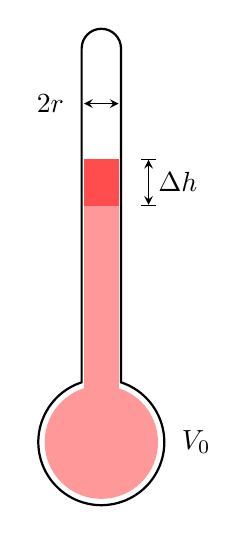
\begin{tikzpicture}[>=stealth]
 \draw[thick] (0.25,5) arc (0:180:0.25) -- (-0.25,0.76) arc (108.2:431.8:0.8) -- cycle;
 \fill[red!40] (0,0) ellipse (0.72 and 0.72);
 \fill[red!40] (-0.22,0.5) rectangle (0.22,3.0);
 \fill[red!70] (-0.22,3.0) rectangle (0.22,3.6);
 \draw[|<->|] (0.6,3.0) -- (0.6,3.6) node[midway, right] {$\Delta h$};
 \draw[<->] (-0.22,4.3) -- (0.22,4.3);
 \node[anchor=east] at (-0.35,4.3) {$2r$};
 \node[anchor=west] at (0.9,0) {$V_0$};
\end{tikzpicture}
\end{center}

Bei einer Temperaturzunahme $\Delta\vartheta$ nimmt das Volumen des Ethanols zu um
\begin{align}
 \Delta V &= \dVtF = \gaEt\cdot\VEt\cdot\dTt = \dVt = \dVtm
\end{align}
mit $\gamma = \gaEtO$ (FoTaBe S.~191; der Wert bei \TtbO\ genügt). Dieses Volumen füllt im Röhrchen einen Zylinder der Höhe $\Delta h$: $\Delta V = \pi\,r^2\,\Delta h$. Damit ist
\begin{align}
 r &= \rTF \\
   &= \sqrt{\frac{\dVt}{\pi\cdot\dhT}} \\
   &= \rT \approx \result{\rTP{-3}{2}}
\end{align}
